\chapter{Planificación}

\fancyhead[R]{5. Planificación}

\noindent\fbox{
	\parbox{\textwidth}{
    En este capítulo se abordará la planificación de las distintas etapas que conforman el proyecto, así como una breve descripción de las mismas. También se tratará la creación de un presupuesto aproximado, y la temporización de las tareas a realizar. 
	}
}
\section{Etapas}

Para comenzar la planificación de la implementación del proyecto, debemos tener en cuenta el tiempo de aprendizaje de las herramientas a utilizar. Se marcarán los siguientes hitos a planificar durante el tiempo en el que se desarrolle el proyecto, así como temporización de los mismos en la siguiente sección y una breve explicación de cada uno de ellos. 

\subsection{Aprendizaje de FreeRTOS}

Para entender las bases de la herramienta que se va a utilizar, es necesario documentarse mediante libros, páginas web de documentación y, si fuera necesario, videoguías.

 Una vez se ha obtenido el suficiente conocimiento de FreeRTOS de manera general, se deben adquirir los fundamentos necesarios para poder trabajar en el entorno de Arduino utilizando la librería que proporciona un port de FreeRTOS denominada \textbf{Arduino FreeRTOS Library}, desarrollada por Phillip Stevens y su equipo, y que ha adquirido licencia del \textbf{MIT} \cite{freertos_arduino}. 

Esta tarea incluye la lectura de la documentación de la librería, el estudio de las funciones adaptadas a Arduino, y la búsqueda de proyectos similares realizados con estas herramientas para su mayor comprensión.

\subsection{Aprendizaje de Processing y la librería ControlP5}

En el ámbito de la interfaz, se debe conocer los fundamentos del lenguaje y entorno de desarrollo \textbf{Processing}, así como el repaso a conceptos y programación en Java, lenguaje en el que está basado. \cite{processing}

Como se ha indicado anteriormente, se utilizará la librería \textbf{ControlP5}, que permitirá una construcción de la interfaz de usuario más rápida e intuitiva. Se deberán conocer las herramientas que provee, la manera en la que está programada, y revisar algunos de los ejemplos que se exponen en su página web \cite{cp5_examples} para cada uno de los subsistemas necesarios para este proyecto.

\begin{figure}[h]
    \centering
    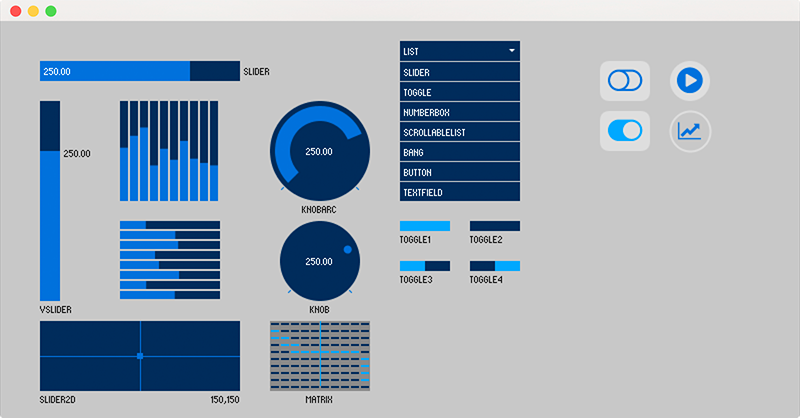
\includegraphics[width=1\textwidth]{imagenes/cp5_examples.png}
    \caption{Imagen con diferentes funcionalidades de ControlP5. Extraído de: \cite{cp5_image}}
\end{figure}

\subsection{Desarrollo de funciones secuenciales sin FREERTOS }

Una vez aprendidos los fundamentos de las herramientas a utilizar, y antes de implementarlas, se debe tener una idea general de las diferentes funciones a incluir en el sistema. Para comenzar con la programación, primero se realizarán de forma secuencial, sin utilizar FreeRTOS, y sin utilizar la comunicación serial. Se comprobará que el funcionamiento sea correcto antes de avanzar a la siguiente etapa. 

\subsection{Desarrollo de funciones concurrentes con FREERTOS}

En esta etapa se adaptarán las funciones desarrolladas anteriormente a FreeRTOS, y se incluirán las medidas pertinentes para asegurar que dichas funciones puedan trabajar de manera concurrente. Se comenzará a trabajar con el puerto serie para mostrar los valores de los sensores, pero sin representarlos de manera gráfica. Se comprobarán los tiempos de respuesta para asegurar que cumple las restricciones de tiempo real. 

\subsection{Desarrollo de interfaz de usuario base sin comunicaciones serie}

Se comenzará a crear la interfaz con Processing, de manera esquemática y sin comunicaciones con Arduino. Se comprobará que todos los módulos responden a los \textit{inputs} del usuario, así como la estructura de dichos módulos divididos en secciones para una mayor comodidad y comprensión.

\subsection{Desarrollo interfaz de usuario con comunicaciones serie}

Utilizando la interfaz base, se añadirá funcionalidad a todos los módulos y comunicación mediante puerto serie con Arduino. También se perfeccionará la interfaz en el aspecto visual. 

\subsection{Depuración, limpieza y documentación del código fuente}

Una vez desarrollada la interfaz de usuario y la programación del sistema, se depurará el código para solucionar los posibles errores que se hayan pasado por alto durante el desarrollo. También se reorganizará y optimizará el código para buscar una mayor eficiencia. 

Tras estos pasos, se realizará una documentación de cada una de las funciones del ámbito de Arduino y se añadirá el archivo de cabeceras. 

\subsection{Montaje en maqueta } 

Como última tarea, y si la temporización real lo permite, se implementará este sistema en una maqueta de un vehículo, que mostrará todas las funciones desarrolladas de una manera más realista en comparación al montaje en \textit{breadboard} que se ha realizado hasta el momento. 

\section{Temporización}


En esta temporización se consideran laborables los días de lunes a sábado, ambos incluidos. Se supone una media de trabajo de tres horas y media al día, sumando un total de veintiún horas a la semana. 

\begin{table}[H]
    \resizebox{\textwidth}{!}{%
    \begin{tabular}{|l|c|c|c|}
    \hline
    \rowcolor[HTML]{DAE8FC} 
    \multicolumn{1}{|c|}{\cellcolor[HTML]{DAE8FC}{\color[HTML]{000000} Tarea}} & {\color[HTML]{000000} \begin{tabular}[c]{@{}c@{}}Tiempo \\ estimado\end{tabular}} & Fecha de inicio & Fecha de finalización \\ \hline
    \textbf{Aprendizaje FreeRTOS} & 1/2 semana & 19/06/2023 & 21/06/2023 \\ \hline
    \textbf{Aprendizaje Processing} & 1/2 semana & 22/06/2023 & 24/06/2023 \\ \hline
    \textbf{Montaje de prototipo} & 3/2 semana & 26/06/2023 & 12/07/2023 \\ \hline
    \textbf{Funciones secuenciales} & 1/2 semana & 26/06/2023 & 28/06/2023 \\ \hline
    \textbf{Funciones concurrentes} & 2 semanas & 29/06/2023 & 12/07/2023 \\ \hline
    \textbf{Interfaz base} & 1 semana & 13/07/2023 & 15/07/2023 \\ \hline
    \textbf{Interfaz con serial} & 1 semana & 17/07/2023 & 23/07/2023 \\ \hline
    \textbf{\begin{tabular}[c]{@{}l@{}}Depuración, limpieza\\ y documentación\end{tabular}} & 1/2 semana & 24/07/2023 & 26/07/2023 \\ \hline
    \textbf{Montaje en maqueta} & 2 semanas & 27/07/2023 & 08/08/2023 \\ \hline
    \end{tabular}%
    }
    \caption[Temporización inicial]{Temporización estimada del proyecto. Elaboración propia}

    \end{table}
    \newpage

    \begin{figure}[H]
        \centering
        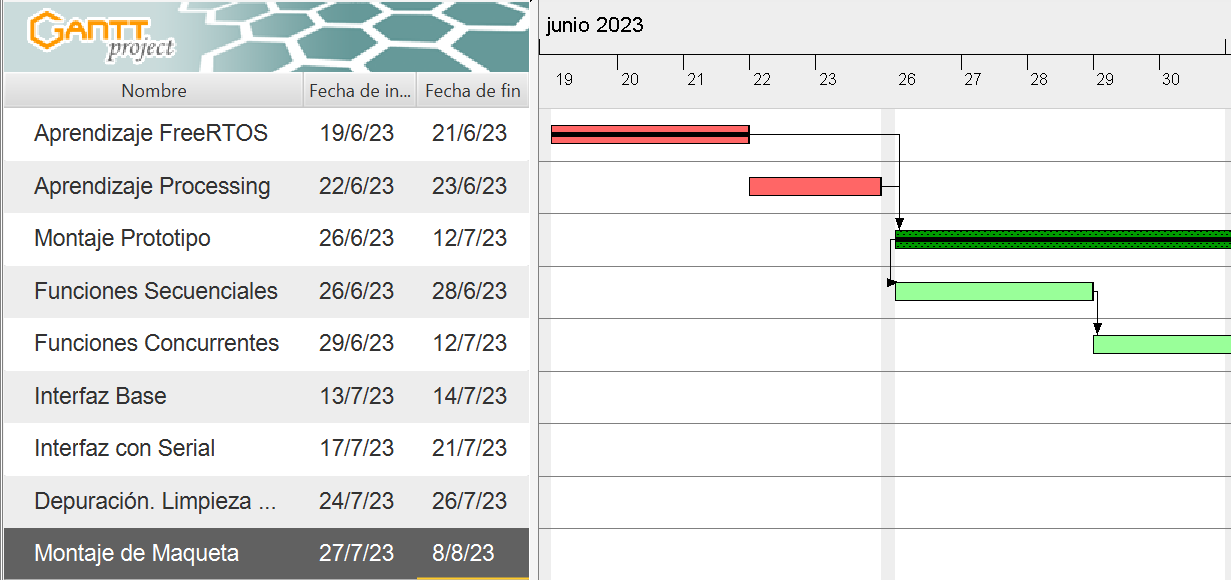
\includegraphics[width=1\textwidth]{imagenes/gantt_base_p1.png}
    \end{figure}
    

    
    \begin{figure}[H]
        \centering
        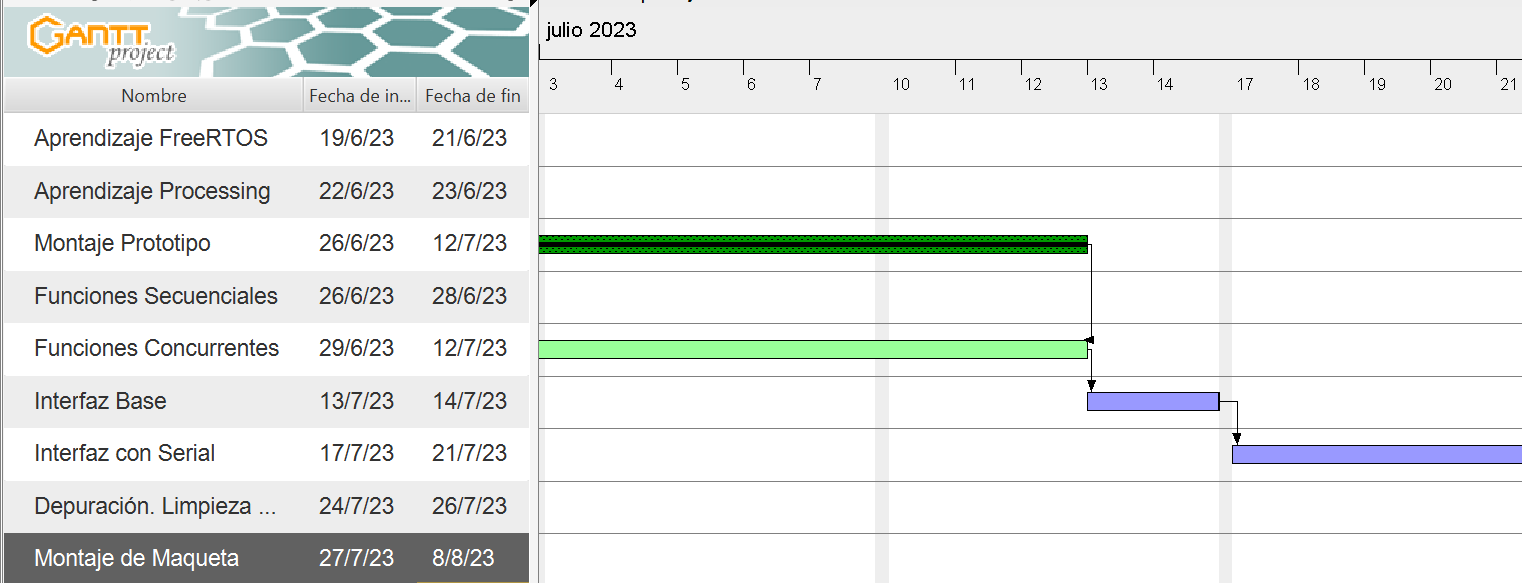
\includegraphics[width=1\textwidth]{imagenes/gantt_base_p2.png}
    \end{figure}
    

    
    \begin{figure}[H]
        \centering
        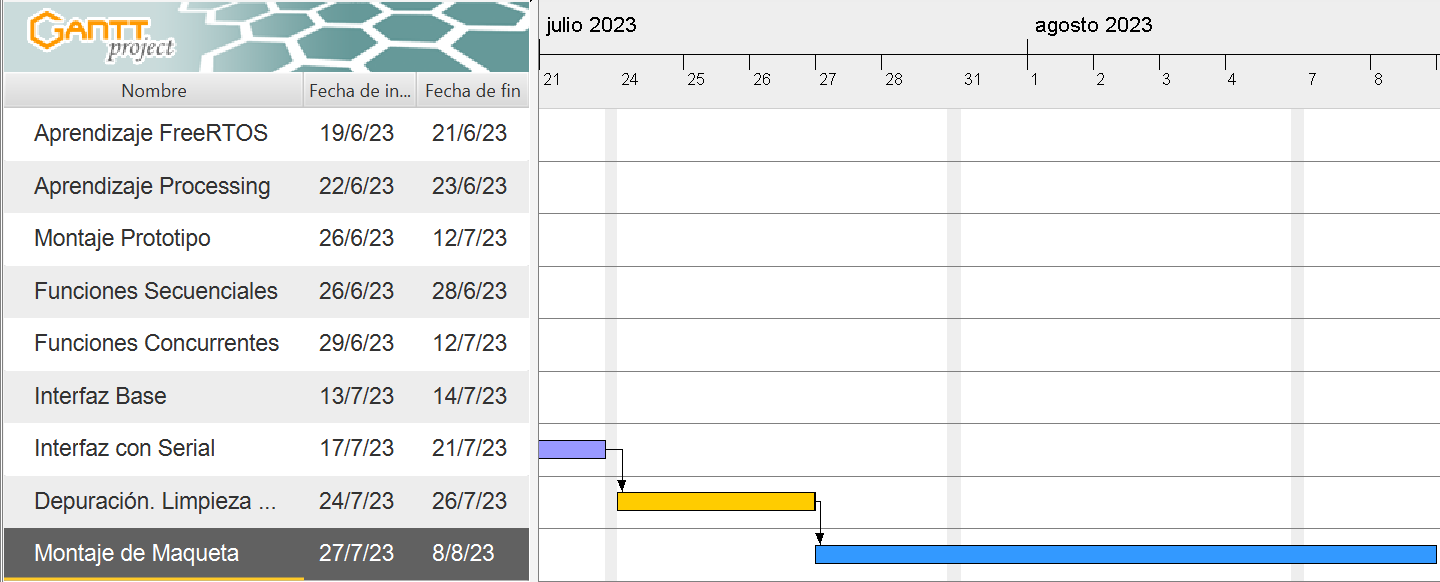
\includegraphics[width=1\textwidth]{imagenes/gantt_base_p3.png}
        \caption{Diagrama de Gantt con las tareas temporizadas. Elaboración propia en GanttProject}
    \end{figure}
    

    \newpage
\section{Presupuesto}

A la hora de calcular el presupuesto necesario para el proyecto, debemos tener en cuenta tres factores principales: \textbf{coste del hardware}, \textbf{coste del software}, y el \textbf{coste de salarios} de los individuos implicados en el proyecto. Ninguno de estos es descartable ni se puede obviar, por lo que esta sección se desglosará en esas tres partes.
\subsection{Coste del hardware}

Al calcular el coste de los componentes que conforman el proyecto se han escogido los precios que se van a pagar en el momento de la planificación, los cuales pueden variar respecto al tiempo en el que se publique este trabajo. 


\begin{table}[H]
    \resizebox{\textwidth}{!}{%
    \begin{tabular}{|l|c|c|c|}
    \hline
    \rowcolor[HTML]{DAE8FC} 
    \multicolumn{1}{|c|}{\cellcolor[HTML]{DAE8FC}{\color[HTML]{000000} \textbf{Componente}}} & \textbf{Unidades} & \textbf{Precio sin I.V.A} & \textbf{Precio con I.V.A} \\ \hline
    \textbf{Placa Arduino Mega 2560 R3 (clon)} & 1 ud & 20,90€ & 26,45€ \\ \hline
    \textbf{LEDs variadas (25 uds)} & 25 uds & 1,98€ & 2,50€ \\ \hline
    \textbf{Resistencias variadas (50 uds)} & 50 uds & 1,98€ & 2,50€ \\ \hline
    \textbf{Batería 9V 650mAh Li-ion} & 2 uds & 21,32€ & 26,99€ \\ \hline
    \textbf{Motor DC} & 2 uds & 7,82€ & 9,90€ \\ \hline
    \textbf{Módulo L298N} & 1 ud & 3,94€ & 4,99€ \\ \hline
    \textbf{Termistor 10k} & 2 uds & 3,15€ & 3,99€ \\ \hline
    \textbf{Cables M-M, M-F, F-F} & 100 uds & 1,98€ & 2,50€ \\ \hline
    \textbf{Maqueta coche Mustang Shelby} & 1 ud & 28,43€ & 35,99€ \\ \hline
    \textbf{Cable USB-A a USB-B de 2 metros} & 1 ud & 7,81€ & 9,99€ \\ \hline
    \multicolumn{2}{|l|}{\textbf{Total}} & 99,31€ & 125,8€ \\ \hline
    \end{tabular}%
    }
    \caption[Presupuesto de componentes]{Lista de componentes con coste. Elaboración propia}

    \end{table}


\subsection{Coste del software}

En esta sección se describirán los costes de los programas utilizados, aunque al darse prioridad al software libre y gratuito, el coste de estas herramientas siempre será cero, exceptuando Windows por la necesidad de este sistema operativo en el ordenador que se está utilizando para otras funciones.

\begin{table}[H]
    \resizebox{\textwidth}{!}{%
    \begin{tabular}{|l|c|l|l|c|}
    \cline{1-2} \cline{4-5}
    \multicolumn{1}{|c|}{\cellcolor[HTML]{DAE8FC}{\color[HTML]{000000} \textbf{Programa / Recurso}}} & \cellcolor[HTML]{DAE8FC}\textbf{Precio licencia} &  & \cellcolor[HTML]{DAE8FC}{\color[HTML]{000000} \textbf{Programa / Recurso}} & \multicolumn{1}{l|}{\cellcolor[HTML]{DAE8FC}{\color[HTML]{000000} \textbf{Precio licencia}}} \\ \cline{1-2} \cline{4-5} 
    \textbf{Arduino IDE} & 0€ &  & \textbf{TexLive} & 0€ \\ \cline{1-2} \cline{4-5} 
    \textbf{FreeRTOS} & 0€ &  & \textbf{GIMP} & 0€ \\ \cline{1-2} \cline{4-5} 
    \textbf{Processing} & 0€ &  & \textbf{GitHub} & 0€ \\ \cline{1-2} \cline{4-5} 
    \textbf{Visual Studio Code} & 0€ &  & \textbf{Mozilla Firefox} & 0€ \\ \cline{1-2} \cline{4-5} 
    \textbf{Atom} & 0€ &  & \textbf{Licencia Windows} & 18€ \\ \cline{1-2} \cline{4-5} 
    \textbf{Tinkercad} & 0€ & & &  \\ \cline{1-2} \cline{4-5}
    \end{tabular}%
    }
    \caption[Presupuesto de software]{Lista de software utilizado con coste. Elaboración propia}
    \end{table}


\subsection{Coste de salarios}

Una vez hallados los costes de software y hardware, se debe estimar el coste dedicado a remunerar los servicios de los diferentes integrantes humanos del proyecto. 

Los salarios medios se han extraído de la plataforma GlassDoor, con lo que se ha calculado el salario por hora de los puestos, asumiendo que dichos puestos estuvieran activos un total de cuarenta horas a la semana, cuatro semanas por mes, durante doce meses. 

\begin{table}[H]
    \resizebox{\textwidth}{!}{%
    \begin{tabular}{|l|l|l|l|l|l|}
    \hline
    \rowcolor[HTML]{DAE8FC} 
    \multicolumn{1}{|c|}{\cellcolor[HTML]{DAE8FC}{\color[HTML]{000000} \textbf{Puesto de trabajo}}} & \multicolumn{1}{c|}{\cellcolor[HTML]{DAE8FC}\textbf{\begin{tabular}[c]{@{}c@{}}Salario\\  por hora\end{tabular}}} & \multicolumn{1}{c|}{\cellcolor[HTML]{DAE8FC}{\color[HTML]{000000} \textbf{\begin{tabular}[c]{@{}c@{}}Horas por\\ semana\end{tabular}}}} & \multicolumn{1}{c|}{\cellcolor[HTML]{DAE8FC}\textbf{\begin{tabular}[c]{@{}c@{}}Semanas\\  de Trabajo\end{tabular}}} & \multicolumn{1}{c|}{\cellcolor[HTML]{DAE8FC}\textbf{\begin{tabular}[c]{@{}c@{}}Total\\ de horas\end{tabular}}} & \multicolumn{1}{c|}{\cellcolor[HTML]{DAE8FC}\textbf{\begin{tabular}[c]{@{}c@{}}Salario\\ Total\end{tabular}}} \\ \hline
    \textbf{\begin{tabular}[c]{@{}l@{}}Ingeniero de\\ Sistemas Empotrados\end{tabular}} & 17,19€/h & 21 horas & 7,5 sem & 157,5 horas & 2707,42€ \\ \hline
    \textbf{\begin{tabular}[c]{@{}l@{}}Desarrollador de \\ interfaces de usuario\end{tabular}} & 14,73€/h & 21 horas & 2 sem & 42 horas & 618,66€ \\ \hline

    \textbf{\begin{tabular}[c]{@{}l@{}}Total del proyecto\end{tabular}} &   & 21 horas & 9,5 sem & 299,5 horas & 3.326,08€ \\ \hline
    \end{tabular}%
    
    }
    \caption[Presupuesto de salarios]{Lista de salarios requeridos para el proyecto. Elaboración propia}

    \end{table}

    \subsection{Coste total}

\begin{table}[H]
    \begin{tabular}{|l|l|l|l|}
    \hline
    \rowcolor[HTML]{DAE8FC} 
    \multicolumn{1}{|c|}{\cellcolor[HTML]{DAE8FC}{\color[HTML]{000000} \textbf{Área del presupuesto}}} & \multicolumn{1}{c|}{\cellcolor[HTML]{DAE8FC}\textbf{Coste}} & \multicolumn{1}{c|}{\cellcolor[HTML]{DAE8FC}{\color[HTML]{000000} \textbf{\begin{tabular}[c]{@{}c@{}}Suma\\ Acumulada\end{tabular}}}} & \multicolumn{1}{c|}{\cellcolor[HTML]{DAE8FC}\textbf{\begin{tabular}[c]{@{}c@{}}Porcentaje\\ del total\end{tabular}}} \\ \hline
    \textbf{Coste Hardware} & 125,80€ & 125,80€ & 3,64\% \\ \hline
    \textbf{Coste Software} & 0€ & 125,80€ & 0\% \\ \hline
    \textbf{Coste Salarios} & 3.326,08€ & 3.451,88 & 96,36\% \\ \hline
    \textbf{Valor Acumulado} & 3.451,88€ & 3.451,88€ & 100\% \\ \hline
    \end{tabular}%

    \caption[Presupuesto total]{Suma total de presupuestos del proyecto. Elaboración propia}
  

    \end{table}

    Si bien el coste del hardware utilizado puede parecer alto, no es comparable al coste de los salarios del equipo de desarrollo pues, aunque no se pueda observar de manera física, el tiempo que conllevan proyectos de este calibre y superiores, requieren de una gran cantidad de horas de trabajo. 
